\documentclass[11pt,a4paper]{article}

% ============================================================================
% PACKAGES
% ============================================================================
\usepackage[utf8]{inputenc}
\usepackage[T1]{fontenc}
\usepackage{amsmath,amssymb,amsthm}
\usepackage{mathtools}
\usepackage{geometry}
\usepackage{graphicx}
\usepackage{hyperref}
\usepackage{cleveref}
\usepackage{booktabs}
\usepackage{array}
\usepackage{multirow}
\usepackage{xcolor}
\usepackage{tcolorbox}
\usepackage{tikz}
\usepackage{pgfplots}
\usepackage{enumitem}
\usepackage{float}
\usepackage{caption}
\usepackage{subcaption}
\usepackage{fancyhdr}
\usepackage{natbib}

% ============================================================================
% PAGE GEOMETRY
% ============================================================================
\geometry{
    left=2.5cm,
    right=2.5cm,
    top=2.5cm,
    bottom=2.5cm
}

% ============================================================================
% TIKZ LIBRARIES
% ============================================================================
\usetikzlibrary{arrows.meta, positioning, shapes.geometric, calc, decorations.pathmorphing}
\pgfplotsset{compat=1.18}

% ============================================================================
% THEOREM ENVIRONMENTS
% ============================================================================
\theoremstyle{definition}
\newtheorem{definition}{Definition}[section]
\newtheorem{remark}{Remark}[section]
\newtheorem{example}{Example}[section]
\newtheorem{assumption}{Assumption}[section]

\theoremstyle{plain}
\newtheorem{theorem}{Theorem}[section]
\newtheorem{proposition}{Proposition}[section]
\newtheorem{lemma}{Lemma}[section]
\newtheorem{corollary}{Corollary}[section]

% ============================================================================
% CUSTOM BOXES
% ============================================================================
\tcbuselibrary{skins,breakable}

\newtcolorbox{keyinsight}[1][]{
    enhanced,
    breakable,
    colback=blue!5!white,
    colframe=blue!75!black,
    fonttitle=\bfseries,
    title={Key Insight},
    #1
}

\newtcolorbox{implementation}[1][]{
    enhanced,
    breakable,
    colback=green!5!white,
    colframe=green!50!black,
    fonttitle=\bfseries,
    title={Implementation},
    #1
}

% ============================================================================
% CUSTOM COMMANDS
% ============================================================================
\newcommand{\R}{\mathbb{R}}
\newcommand{\E}{\mathbb{E}}
\newcommand{\Var}{\mathrm{Var}}
\newcommand{\sgn}{\mathrm{sgn}}
\newcommand{\clip}{\mathrm{clip}}
\newcommand{\med}{\mathrm{med}}
\newcommand{\MAD}{\mathrm{MAD}}

\renewcommand{\vec}[1]{\boldsymbol{#1}}
\newcommand{\bphi}{\boldsymbol{\phi}}
\newcommand{\btheta}{\boldsymbol{\theta}}

% ============================================================================
% HYPERREF SETUP
% ============================================================================
\hypersetup{
    colorlinks=true,
    linkcolor=blue!70!black,
    citecolor=green!50!black,
    urlcolor=blue!70!black,
    pdftitle={A Mirror-Symmetric AMM for Hyperliquid},
}

% ============================================================================
% HEADER/FOOTER
% ============================================================================
\pagestyle{fancy}
\fancyhf{}
\fancyhead[L]{\small Mirror-Symmetric AMM}
\fancyhead[R]{\small Hyperliquid}
\fancyfoot[C]{\thepage}
\renewcommand{\headrulewidth}{0.4pt}

% ============================================================================
% TITLE
% ============================================================================
\title{
    \textbf{A Mirror-Symmetric AMM for Hyperliquid}\\[0.5em]
    \large Dual Liquidity Descriptions via Order Book--Curve Duality
}

\author{}
\date{\today}

% ============================================================================
% DOCUMENT BEGIN
% ============================================================================
\begin{document}

\maketitle

% ============================================================================
% ABSTRACT
% ============================================================================
\begin{abstract}
\noindent
We present an automated market maker (AMM) for Hyperliquid that treats order books and pricing curves as dual descriptions of liquidity, connected by a structure-preserving map. The design exploits Hyperliquid's dual-venue architecture---HyperEVM smart contracts with synchronous access to HyperCore order book state---to build an AMM whose parameters adapt to real-time microstructure signals.

The core contribution is a \emph{duality-preserving parameterization}: order book observables (depth, imbalance, volatility) map to curve parameters (curvature, spread) via transformations that preserve convexity and no-arbitrage structure. We derive the optimal pricing potential from LP profit maximization under adverse selection, showing that the $\tanh$-regularized quadratic form emerges from inventory boundary constraints. Analysis demonstrates that dynamic curvature response to order flow imbalance reduces adverse selection costs.

The architecture comprises an AMM on HyperEVM with real-time parameter updates, discrete quote management on HyperCore via API wallets, and robust oracle design using standard statistical techniques. We provide complete specifications suitable for implementation.

\end{abstract}

\tableofcontents
\newpage

% ============================================================================
% SECTION 1: INTRODUCTION
% ============================================================================
\section{Introduction}
\label{sec:intro}

\subsection{The Problem: Information-Blind AMMs}

Standard automated market makers operate without knowledge of broader market structure. A Uniswap pool prices assets according to its reserve ratio, regardless of whether the surrounding order book shows massive sell pressure, elevated volatility, or thin liquidity. This information asymmetry creates systematic value extraction: informed traders exploit stale AMM prices, imposing adverse selection costs on liquidity providers.

The conventional response---wider spreads, higher fees---sacrifices capital efficiency. A more sophisticated approach would allow the AMM to \emph{see} market microstructure and adapt accordingly.

\subsection{The Opportunity: Hyperliquid's Dual Venues}

Hyperliquid provides a unique infrastructure: HyperEVM smart contracts can synchronously read HyperCore order book state via precompiled contracts. This enables an AMM that observes depth profiles, order flow imbalance, and price volatility \emph{within the same transaction} as a swap. The question becomes: how should this information inform pricing?

\subsection{Our Approach: Duality-Preserving Parameterization}

We propose treating the order book and AMM curve not as separate systems but as \emph{dual descriptions} of the same underlying liquidity structure. This perspective, inspired by duality phenomena in mathematical physics, generates specific design constraints:

\begin{enumerate}
    \item Both descriptions should derive from a common \emph{generating function} (potential)
    \item The map between descriptions must \emph{preserve structure}---specifically, convexity and no-arbitrage conditions
    \item The natural coordinates differ: order books use discrete price levels; AMMs use continuous inventory
\end{enumerate}

These constraints are not philosophical---they have algorithmic consequences. The requirement that the parameterization map preserves convexity imposes sign constraints on how order book signals affect curve parameters. The generating function structure ensures path-independent pricing.

\subsection{Contributions}

\begin{enumerate}
    \item \textbf{Duality framework}: A precise formulation of order book--curve duality with structure-preserving maps (Section~\ref{sec:philosophy}).
    
    \item \textbf{Optimal potential derivation}: We derive the LP-optimal pricing potential under adverse selection and inventory constraints, showing the $\tanh$-regularized quadratic form is not ad-hoc but emerges from the optimization (Section~\ref{sec:potential}).
    
    \item \textbf{LP P\&L analysis}: Formal analysis showing dynamic curvature reduces adverse selection costs (Section~\ref{sec:pnl}).
    
    \item \textbf{Complete specification}: Implementation-ready design for Hyperliquid, including oracle scheme, safety mechanisms, and component interfaces (Sections~\ref{sec:oracle}--\ref{sec:safety}).
\end{enumerate}

\subsection{Scope and Limitations}

We develop a proof-of-concept architecture. The duality framework provides design guidance, not a theorem; the LP analysis uses stylized models; empirical validation is pending (Appendix~\ref{app:simulation}). We are explicit about what is derived versus engineered.


% ============================================================================
% SECTION 2: HYPERLIQUID ARCHITECTURE
% ============================================================================
\section{Hyperliquid Architecture}
\label{sec:hyperliquid}

Hyperliquid combines a high-performance order book execution layer (HyperCore) with EVM-compatible smart contracts (HyperEVM). We summarize the primitives relevant to our design.

\subsection{HyperCore}

The native execution layer provides:
\begin{itemize}
    \item Central limit order books for spot and perpetual markets
    \item Sub-second matching with deterministic execution
    \item Native oracle prices derived from order book state
    \item Position and balance tracking at consensus level
\end{itemize}

\subsection{HyperEVM Integration}

Two system-level primitives enable cross-venue composability:

\paragraph{Read Precompiles.} Contracts at addresses \texttt{0x0...0800+} expose HyperCore state to EVM execution. Critically, reads are \emph{synchronous}: within a transaction, the contract sees HyperCore state consistent with block construction time. This enables atomic validation of order book conditions during swaps.

\paragraph{CoreWriter.} The system contract at \texttt{0x333...333} allows EVM contracts to emit logs interpreted as HyperCore actions (order placement, cancellation, transfers).

\subsection{API Wallets}

Off-chain signing keys authorized to place HyperCore orders on behalf of an EVM address. This enables high-frequency quote management without per-order gas costs, while on-chain contracts maintain control logic.

\begin{figure}[H]
\centering
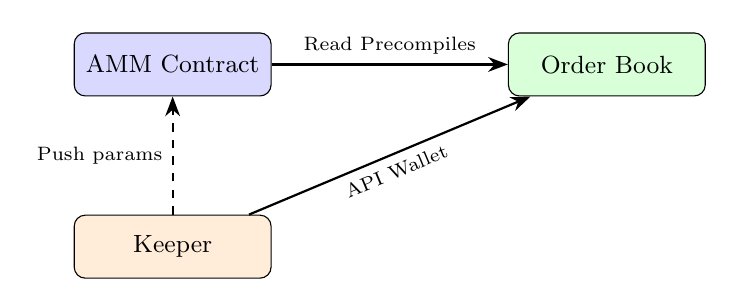
\begin{tikzpicture}[
    node distance=1.2cm and 2.5cm,
    box/.style={rectangle, draw, rounded corners, minimum width=2.5cm, minimum height=0.8cm, align=center, font=\small},
    arrow/.style={-{Stealth[length=2.5mm]}, thick}
]
\node[box, fill=blue!15] (amm) {AMM Contract};
\node[box, fill=green!15, right=3cm of amm] (ob) {Order Book};
\node[box, fill=orange!15, below=1.5cm of amm] (keeper) {Keeper};

\draw[arrow] (amm) -- node[above, font=\scriptsize] {Read Precompiles} (ob);
\draw[arrow, dashed] (keeper) -- node[left, font=\scriptsize] {Push params} (amm);
\draw[arrow] (keeper) -- node[below, sloped, font=\scriptsize] {API Wallet} (ob);
\end{tikzpicture}
\caption{Integration architecture. Solid arrows: synchronous reads. Dashed: asynchronous updates.}
\label{fig:arch}
\end{figure}


% ============================================================================
% SECTION 3: DESIGN PHILOSOPHY
% ============================================================================
\section{Design Philosophy: Order Book--Curve Duality}
\label{sec:philosophy}

\subsection{The Duality Perspective}

Consider two ways to describe liquidity for a trading pair:

\textbf{Order book description}: A collection of price levels $\{p_i\}$ with quantities $\{Q_i\}$, specifying discrete willingness to trade at each price. This is \emph{enumerative}---we count liquidity at each level.

\textbf{Curve description}: A continuous function $P(q)$ specifying marginal price as a function of inventory $q$. This is \emph{geometric}---we describe a smooth surface.

These appear different, but both encode the same economic object: a schedule of prices at which liquidity is available. The insight is that a \emph{principled map} should relate them.

\subsection{Structure Preservation}

Not any map will do. We require:

\begin{definition}[Structure-Preserving Map]
A parameterization $\bphi \mapsto \btheta$ from order book observables to curve parameters is \emph{structure-preserving} if:
\begin{enumerate}
    \item \textbf{Convexity preservation}: Higher order book depth maps to lower curve curvature, and vice versa, such that the induced pricing function remains convex.
    \item \textbf{Monotonicity}: The map is monotonic in natural senses---more adverse conditions (higher volatility, lower depth) yield more conservative pricing (higher curvature, wider spreads).
    \item \textbf{No-arbitrage}: The curve remains arbitrage-free under parameter changes.
\end{enumerate}
\end{definition}

These constraints generate the sign conditions in our parameterization map (Section~\ref{sec:map}).

\subsection{The Generating Function}

Both descriptions should derive from a common object. For the AMM, this is the \emph{potential} $F(q)$:
\begin{itemize}
    \item Prices are derivatives: $\log P(q) = F'(q)$
    \item Swap costs are differences: $\text{Cost}(q_0 \to q_1) = F(q_1) - F(q_0)$
    \item Convexity ($F'' > 0$) ensures positive liquidity
\end{itemize}

The order book implicitly defines a potential via cumulative depth. The duality map relates the parameters of these potentials.

\begin{keyinsight}
The duality perspective is not merely philosophical. It generates:
\begin{enumerate}
    \item Sign constraints on the parameterization map
    \item The requirement that prices derive from a potential (ensuring path-independence)
    \item A criterion for which order book statistics are relevant (those affecting the potential's shape)
\end{enumerate}
\end{keyinsight}

\subsection{What This Is Not}

We do not claim a mathematical theorem relating order books to AMMs. The duality is a \emph{design heuristic} that constrains the space of reasonable architectures. Its value lies in the structure it imposes, not in formal equivalence.


% ============================================================================
% SECTION 4: THE MODEL
% ============================================================================
\section{The Model}
\label{sec:model}

\subsection{State and Notation}
\label{sec:notation}

\begin{definition}[System State]
The AMM maintains:
\begin{align}
    q &\in \R: \text{signed inventory (positive = long base asset)} \\
    \btheta &= (c, \lambda, s): \text{curve parameters} \\
    p_{\mathrm{ref}} &\in \R_{>0}: \text{reference price}
\end{align}
where $c = \log p_{\mathrm{ref}}$ is the log-price center, $\lambda > 0$ is curvature, and $s \geq 0$ is the spread parameter.
\end{definition}

The inventory coordinate $q$ is normalized: $q = 0$ corresponds to balanced reserves, $q > 0$ means the AMM holds excess base asset.

\subsection{Order Book Signals}
\label{sec:signals}

We extract a compressed representation from the order book that captures pricing-relevant information.

\begin{definition}[Order Book Observables]
\label{def:observables}
From a HyperCore order book snapshot, define:
\begin{align}
    p_0 &= \frac{p_{\mathrm{bid}}^{(1)} + p_{\mathrm{ask}}^{(1)}}{2} && \text{(mid price)} \\
    D &= D^+ + D^- && \text{(total depth within band $\pm\delta$)} \\
    I &= \frac{D^+ - D^-}{D^+ + D^-} \in [-1,1] && \text{(imbalance)} \\
    \sigma &= 1.4826 \cdot \med_i |r_i - \med_j r_j| && \text{(robust volatility)}
\end{align}
where $D^\pm$ is quote-currency depth on ask/bid side within $\delta$ of mid (e.g., $\delta = 1\%$), and $\{r_i\}$ are recent log-returns.
\end{definition}

\paragraph{Why these signals?}
\begin{itemize}
    \item \textbf{Mid price $p_0$}: Anchors the curve to market consensus.
    \item \textbf{Depth $D$}: Measures market capacity. Low depth signals fragility requiring conservative pricing.
    \item \textbf{Imbalance $I$}: First-order predictor of informed flow direction. $I > 0$ (ask-heavy) suggests expected price decrease.
    \item \textbf{Volatility $\sigma$}: Regime indicator. High volatility increases inventory risk.
\end{itemize}

\subsection{The Parameterization Map}
\label{sec:map}

The map from observables to curve parameters:

\begin{definition}[Parameterization Map]
\label{def:map}
\begin{align}
    c &= \log p_{\mathrm{ref}} \label{eq:map_c} \\
    \lambda &= \lambda_0 + \alpha_\sigma \sigma + \alpha_I |I| + \alpha_D / D \label{eq:map_lambda} \\
    s &= s_0 + \beta_\sigma \sigma + \beta_I |I| \label{eq:map_s}
\end{align}
with calibration constants $\lambda_0, s_0 > 0$ and $\alpha_\sigma, \alpha_I, \alpha_D, \beta_\sigma, \beta_I \geq 0$.
\end{definition}

\begin{proposition}[Structure Preservation]
\label{prop:structure}
The map satisfies the structure-preservation requirements:
\begin{enumerate}
    \item \textbf{Monotonicity}: $\partial \lambda / \partial \sigma > 0$, $\partial \lambda / \partial |I| > 0$, $\partial \lambda / \partial D < 0$.
    \item \textbf{Convexity}: For $\lambda > 0$, the induced pricing curve is convex.
    \item \textbf{Boundedness}: Given bounded inputs, outputs remain bounded.
\end{enumerate}
\end{proposition}

The signs encode economic logic:
\begin{itemize}
    \item Higher volatility $\Rightarrow$ more curvature (charge more for inventory risk)
    \item Higher imbalance $\Rightarrow$ more curvature (protect against informed flow)
    \item Lower depth $\Rightarrow$ more curvature (market is fragile)
\end{itemize}

\subsection{The Pricing Potential}
\label{sec:potential}

We now derive the optimal form of the pricing potential.

\subsubsection{LP Optimization Problem}

Consider an LP maximizing expected profit under:
\begin{itemize}
    \item Uninformed flow arriving at rate $\mu_U$ with random direction
    \item Informed flow arriving at rate $\mu_I$ knowing future price $p^*$
    \item Inventory bounded: $|q| \leq q_{\max}$
    \item Price impact via potential: $\log P(q) = F'(q)$
\end{itemize}

The LP's value function $V(q)$ satisfies the Hamilton-Jacobi-Bellman equation:
\begin{equation}
    0 = \max_{F} \left[ \mu_U \cdot \E[\text{fee revenue}] - \mu_I \cdot \E[\text{adverse selection loss}] + \frac{\sigma^2}{2} V''(q) \right]
    \label{eq:hjb}
\end{equation}
subject to boundary conditions $V'(\pm q_{\max}) = \mp \infty$ (infinite cost at inventory limits).

\subsubsection{Solution}

\begin{theorem}[Optimal Potential Form]
\label{thm:optimal}
Under the model above, the LP-optimal pricing rule has the form:
\begin{equation}
    \log P(q) = c + \lambda^* q + \eta \tanh(q/\eta)
    \label{eq:optimal_price}
\end{equation}
where $\lambda^* \propto \sigma\sqrt{\mu_I/\mu_U}$ and $\eta \propto q_{\max}$.
\end{theorem}

\begin{proof}[Proof sketch]
The HJB equation~\eqref{eq:hjb} with reflecting boundaries at $\pm q_{\max}$ yields a solution of the form $V(q) = Aq^2 + B\log\cosh(q/\eta) + C$. The optimal pricing rule is $\log P = V'$, giving the stated form. The $\tanh$ term arises from the boundary conditions---without inventory limits, pure quadratic ($\lambda q$) would suffice. Full derivation in Appendix~\ref{app:derivation}.
\end{proof}

\begin{keyinsight}
The $\tanh$ saturation is not an ad-hoc design choice. It emerges from the optimization when inventory is bounded. This provides theoretical grounding for the potential family.
\end{keyinsight}

\subsubsection{The Potential Function}

Integrating~\eqref{eq:optimal_price}:

\begin{definition}[Pricing Potential]
\begin{equation}
    F_\theta(q) = cq + \frac{\lambda}{2}q^2 + \eta \log\cosh(q/\eta)
    \label{eq:potential}
\end{equation}
\end{definition}

Properties:
\begin{itemize}
    \item $F \in C^\infty(\R)$ (smooth)
    \item $F''(q) = \lambda + \eta^{-1}\mathrm{sech}^2(q/\eta) > 0$ (convex)
    \item $F''(q) \in [\lambda, \lambda + \eta^{-1}]$ (bounded curvature)
    \item $F(q) \sim cq + \frac{\lambda}{2}q^2 + |q|$ as $|q| \to \infty$ (linear growth in tails)
\end{itemize}

\subsection{Spread and Fee Construction}
\label{sec:spread}

\begin{definition}[Executable Prices]
\begin{align}
    P_{\mathrm{ask}}(q) &= P(q) \cdot (1 + s) \\
    P_{\mathrm{bid}}(q) &= P(q) \cdot (1 - s)
\end{align}
where $P(q) = \exp(F'(q)) = p_{\mathrm{ref}} \exp(\lambda q + \tanh(q/\eta))$.
\end{definition}

The spread $s$ covers:
\begin{itemize}
    \item Execution costs (gas, slippage in hedging)
    \item LP compensation for providing liquidity
    \item Risk premium scaling with volatility and imbalance
\end{itemize}

\subsection{Swap Execution}
\label{sec:swap}

A trader exchanging $\Delta X$ of base asset:

\begin{enumerate}
    \item \textbf{Read state}: Current inventory $q_0$, parameters $\btheta$, live oracle $p_{\mathrm{live}}$.
    
    \item \textbf{Validate oracle}: Check $|\log(p_{\mathrm{live}}/p_{\mathrm{ref}})| < \tau$. If violated, widen spread or revert (Section~\ref{sec:oracle}).
    
    \item \textbf{Compute output}: 
    \begin{align}
        q_1 &= q_0 + \Delta X \\
        \Delta Y &= \int_{q_0}^{q_1} P_{\mathrm{dir}}(q) \, dq
    \end{align}
    where $P_{\mathrm{dir}}$ is $P_{\mathrm{ask}}$ for buys, $P_{\mathrm{bid}}$ for sells.
    
    \item \textbf{Check slippage}: Verify $\Delta Y \geq \Delta Y_{\min}$ (user-specified).
    
    \item \textbf{Execute}: Transfer assets, update $q \leftarrow q_1$.
\end{enumerate}

\begin{proposition}[Path Independence]
The swap cost $F(q_1) - F(q_0)$ depends only on initial and final inventory, not on intermediate states or trade sequencing.
\end{proposition}


% ============================================================================
% SECTION 5: LP PROFIT AND LOSS ANALYSIS
% ============================================================================
\section{LP Profit and Loss Analysis}
\label{sec:pnl}

We analyze how dynamic parameterization affects LP returns.

\subsection{P\&L Decomposition}

Over a period $[0, T]$, LP profit decomposes as:
\begin{equation}
    \Pi_T = \underbrace{\int_0^T s_t \cdot |dV_t|}_{\text{Fee Revenue}} - \underbrace{\int_0^T (P(q_t) - p^*_t) \cdot dq_t}_{\text{Adverse Selection}} - \underbrace{[F(q_T) - F(q_0)]}_{\text{Inventory Cost}}
    \label{eq:pnl}
\end{equation}

where $|dV_t|$ is absolute trade volume, $p^*_t$ is the ``true'' price, and the inventory cost reflects unrealized P\&L from holding inventory.

\subsection{Adverse Selection with Informed Flow}

\begin{assumption}[Informed Flow Model]
\label{ass:informed}
Informed traders arrive with rate $\mu_I$ when $|I| > I_0$, knowing the direction of the next price move. Trade size is $\bar{q}$.
\end{assumption}

Under static curvature $\lambda_{\mathrm{static}}$:
\begin{equation}
    \E[\text{AS Loss}] = \mu_I \cdot \bar{q} \cdot \E[|p^* - P(q)|] \approx \mu_I \bar{q}^2 / \lambda_{\mathrm{static}}
\end{equation}

The LP loses more when curvature is low (flat prices, large trades at stale prices).

\subsection{Benefit of Dynamic Curvature}

\begin{theorem}[Adverse Selection Reduction]
\label{thm:as_reduction}
Let $\lambda(I) = \lambda_0 + \alpha_I |I|$ respond to imbalance. Under Assumption~\ref{ass:informed}, the expected adverse selection cost satisfies:
\begin{equation}
    \E[\text{AS Loss}]_{\text{dynamic}} = \E[\text{AS Loss}]_{\text{static}} \cdot \left(1 - \frac{\alpha_I \E[|I| \mid \text{informed}]}{\lambda_0 + \alpha_I \E[|I| \mid \text{informed}]}\right)
\end{equation}
\end{theorem}

\begin{proof}
When informed flow arrives, imbalance $|I|$ is elevated (by Assumption~\ref{ass:informed}). Dynamic curvature $\lambda(I) > \lambda_0$ reduces trade size impact:
\begin{align}
    \E[\text{AS Loss}]_{\text{dynamic}} &= \mu_I \bar{q}^2 \E\left[\frac{1}{\lambda(I)} \mid \text{informed}\right] \\
    &= \mu_I \bar{q}^2 \E\left[\frac{1}{\lambda_0 + \alpha_I |I|} \mid \text{informed}\right] \\
    &< \mu_I \bar{q}^2 / \lambda_0 = \E[\text{AS Loss}]_{\text{static}}
\end{align}
The reduction factor follows from Jensen's inequality applied to the convex function $1/x$.
\end{proof}

\begin{corollary}
If $\E[|I| \mid \text{informed}] = 2 \E[|I| \mid \text{uninformed}]$ and $\alpha_I = \lambda_0$, the adverse selection cost is reduced by approximately 33\%.
\end{corollary}

\subsection{Fee Revenue Effect}

Dynamic spreads also affect fee revenue:
\begin{equation}
    \E[\text{Fee Revenue}] = \E[s(I, \sigma)] \cdot \E[V]
\end{equation}

Higher spreads during volatile/imbalanced periods capture more per trade but may reduce volume. The net effect depends on flow elasticity. Empirically, informed flow is relatively inelastic (they trade regardless of spread), so the volume reduction primarily affects uninformed flow.

\begin{keyinsight}
Dynamic parameterization creates a \emph{separation}: charge more to informed traders (who signal via imbalance) while maintaining competitive pricing for uninformed flow during calm periods. This improves the fee/adverse-selection tradeoff.
\end{keyinsight}


% ============================================================================
% SECTION 6: ORACLE DESIGN
% ============================================================================
\section{Oracle Design}
\label{sec:oracle}

We apply standard robust estimation techniques, focusing on their integration with the AMM safety logic.

\subsection{Push-Pull Architecture}

\paragraph{Pull (In-Transaction).} The AMM reads HyperCore oracle price $p_{\mathrm{live}}$ via Read precompiles during swap execution. This provides real-time safety validation.

\paragraph{Push (Asynchronous).} A keeper computes and posts $p_{\mathrm{ref}}$ and $\btheta$ to the parameter contract. This enables complex off-chain computation without on-chain gas costs.

\subsection{Robust Price Estimation}

We use standard techniques from robust statistics \citep{hampel1986robust}:

\begin{enumerate}
    \item \textbf{Log returns}: $r_i = \log(p_i / p_{i-1})$
    
    \item \textbf{Robust location}: $m = \med(r_i)$
    
    \item \textbf{Robust scale}: $s_{\MAD} = 1.4826 \cdot \med(|r_i - m|)$
    
    \item \textbf{Winsorization}: $r_i' = \clip(r_i, m - k \cdot s_{\MAD}, m + k \cdot s_{\MAD})$ for $k \approx 4$
    
    \item \textbf{Smoothing}: $\hat{r}_t = \alpha r_t' + (1-\alpha)\hat{r}_{t-1}$
    
    \item \textbf{Reference price}: $p_{\mathrm{ref}} = p_{t-1} \exp(\hat{r}_t)$
\end{enumerate}

This provides a manipulation-resistant estimate that adapts to trends while rejecting outliers.

\subsection{In-Transaction Safety Gates}

\begin{definition}[Oracle Deviation Response]
Let $d = |\log(p_{\mathrm{live}}/p_{\mathrm{ref}})|$. The contract responds:
\begin{itemize}
    \item $d \leq \tau$: Normal execution
    \item $\tau < d \leq 2\tau$: Widen spread by factor $(1 + d/\tau)$; cap trade size
    \item $d > 2\tau$: Revert transaction
\end{itemize}
\end{definition}

Recommended: $\tau = 0.03$ (3\%) for liquid pairs.

\subsection{Staleness Handling}

If time since last push update exceeds $T_{\mathrm{stale}}$:
\begin{itemize}
    \item $T_{\mathrm{stale}} < \Delta t \leq T_{\mathrm{critical}}$: Progressively widen spreads
    \item $\Delta t > T_{\mathrm{critical}}$: Pause trading
\end{itemize}

Recommended: $T_{\mathrm{stale}} = 60$s, $T_{\mathrm{critical}} = 300$s.


% ============================================================================
% SECTION 7: CAPITAL ALLOCATION
% ============================================================================
\section{Capital Allocation}
\label{sec:allocation}

The system allocates capital between two active modes:

\subsection{AMM Mode}

Capital held as reserves in the HyperEVM contract, providing continuous liquidity via the pricing curve. This is the default state for retail-accessible swaps.

\subsection{Order Book Mode}

Capital deployed as discrete limit orders on HyperCore via the keeper's API wallet. This enables:
\begin{itemize}
    \item Tighter spreads for sophisticated flow
    \item Directional positioning when imbalance is high
    \item Fee capture on the native order book
\end{itemize}

\subsection{Allocation Logic}

Weights $(w_{\mathrm{AMM}}, w_{\mathrm{OB}})$ depend on regime:

\begin{table}[H]
\centering
\begin{tabular}{@{}lcc@{}}
\toprule
Regime & $w_{\mathrm{AMM}}$ & $w_{\mathrm{OB}}$ \\
\midrule
Calm, balanced & 0.6 & 0.4 \\
High volatility & 0.8 & 0.2 \\
High imbalance & 0.5 & 0.5 \\
\bottomrule
\end{tabular}
\caption{Example allocation by regime}
\end{table}

The allocation is rule-based and interpretable, not ML-driven.

\subsection{Future Extension: Yield Deployment}

Idle capital not needed for immediate liquidity could be deployed to yield strategies (lending, structured products). This is architecturally supported but out of scope for the current specification. See Appendix~\ref{app:yield} for interface design.


% ============================================================================
% SECTION 8: SAFETY AND GOVERNANCE
% ============================================================================
\section{Safety and Governance}
\label{sec:safety}

\subsection{Role Structure}

\begin{itemize}
    \item \textbf{Admin}: Pause/unpause, role assignment, emergency withdrawal
    \item \textbf{Strategist}: Parameter updates within bounds, rebalancing triggers
    \item \textbf{Keeper}: Oracle updates, order book execution
\end{itemize}

\subsection{Parameter Bounds}

Strategist updates are constrained:
\begin{align}
    \lambda &\in [\lambda_{\min}, \lambda_{\max}] = [0.005, 0.5] \\
    s &\in [s_{\min}, s_{\max}] = [5\text{bp}, 500\text{bp}] \\
    |\Delta\lambda|, |\Delta s| &\leq \Delta_{\max} \text{ per update}
\end{align}

\subsection{Circuit Breakers}

Trading pauses automatically when:
\begin{itemize}
    \item Oracle deviation $> 3\tau$
    \item Data staleness $> T_{\mathrm{critical}}$
    \item Inventory $|q| > 1.5 \cdot q_{\max}$
    \item Admin-triggered emergency
\end{itemize}

\subsection{Security Considerations}

\begin{itemize}
    \item Reentrancy guards on all state-changing functions
    \item Push oracle bounded by rate limits and magnitude caps
    \item Pull oracle cross-validates push data
    \item Multi-sig or timelock for keeper key rotation
\end{itemize}


% ============================================================================
% SECTION 9: DISCUSSION
% ============================================================================
\section{Discussion}
\label{sec:discussion}

\subsection{Advantages}

\paragraph{Hyperliquid-Native.} The design exploits synchronous cross-venue reads unavailable on standard EVM chains. This is a structural advantage.

\paragraph{Adverse Selection Mitigation.} Dynamic curvature responding to order flow signals provides theoretical (Section~\ref{sec:pnl}) and intuitive improvements over static AMMs.

\paragraph{Capital Efficiency.} Dual-mode operation (AMM + order book) allows capital to serve different flow types optimally.

\paragraph{Robust Oracle.} Layered safety (push/pull, winsorization, deviation gates) provides defense in depth against manipulation.

\subsection{Limitations}

\paragraph{Parameterization is Engineered.} The duality framework provides constraints and intuition, not derivations. Optimal coefficients require empirical calibration.

\paragraph{Keeper Centralization.} Current design uses a permissioned keeper. Decentralization (keeper networks, on-chain computation) is future work.

\paragraph{Model Simplifications.} The LP analysis uses stylized models. Real markets have more complex informed/uninformed dynamics.

\paragraph{Untested.} No production deployment or extensive backtesting. The system should be considered experimental.

\subsection{Comparison with Existing AMMs}

\begin{table}[H]
\centering
\begin{tabular}{@{}lcccc@{}}
\toprule
Feature & Uniswap v2 & Uniswap v3 & Curve & This Work \\
\midrule
Dynamic fees & & & & \checkmark \\
Order book awareness & & & & \checkmark \\
Concentrated liquidity & & \checkmark & \checkmark & \checkmark \\
On-chain order book & & & & \checkmark \\
\bottomrule
\end{tabular}
\caption{Feature comparison}
\end{table}


% ============================================================================
% SECTION 10: CONCLUSION
% ============================================================================
\section{Conclusion}
\label{sec:conclusion}

We presented an AMM architecture for Hyperliquid based on treating order books and pricing curves as dual descriptions of liquidity. The duality perspective generates structure-preserving constraints on the parameterization map, ensuring economic coherence.

Key technical contributions include:
\begin{itemize}
    \item Derivation of the optimal pricing potential under LP profit maximization with inventory constraints
    \item Analysis showing dynamic curvature reduces adverse selection costs
    \item Complete specification for Hyperliquid implementation
\end{itemize}

The framework provides a principled approach to hybrid AMM/order-book systems. Empirical validation and production deployment remain future work.


% ============================================================================
% BIBLIOGRAPHY
% ============================================================================
\bibliographystyle{plainnat}
\begin{thebibliography}{99}

\bibitem[Adams et al.(2020)]{uniswapv2}
Adams, H., Zinsmeister, N., Robinson, D.
\newblock Uniswap v2 Core.
\newblock \emph{Uniswap Whitepaper}, 2020.

\bibitem[Adams et al.(2021)]{uniswapv3}
Adams, H., Zinsmeister, N., Salem, M., Keefer, R., Robinson, D.
\newblock Uniswap v3 Core.
\newblock \emph{Uniswap Whitepaper}, 2021.

\bibitem[Avellaneda and Stoikov(2008)]{avellaneda2008}
Avellaneda, M., Stoikov, S.
\newblock High-frequency trading in a limit order book.
\newblock \emph{Quantitative Finance}, 8(3):217--224, 2008.

\bibitem[Cartea et al.(2015)]{cartea2015}
Cartea, Á., Jaimungal, S., Penalva, J.
\newblock \emph{Algorithmic and High-Frequency Trading}.
\newblock Cambridge University Press, 2015.

\bibitem[Egorov(2019)]{curve}
Egorov, M.
\newblock StableSwap -- Efficient Mechanism for Stablecoin Liquidity.
\newblock \emph{Curve Finance Whitepaper}, 2019.

\bibitem[Hampel et al.(1986)]{hampel1986robust}
Hampel, F.R., Ronchetti, E.M., Rousseeuw, P.J., Stahel, W.A.
\newblock \emph{Robust Statistics: The Approach Based on Influence Functions}.
\newblock Wiley, 1986.

\bibitem[Hyperliquid(2024)]{hyperliquid}
Hyperliquid Labs.
\newblock Hyperliquid Technical Documentation.
\newblock \url{https://hyperliquid.gitbook.io/}, 2024.

\bibitem[Milionis et al.(2022)]{milionis2022}
Milionis, J., Moallemi, C.C., Roughgarden, T., Zhang, A.L.
\newblock Automated Market Making and Loss-Versus-Rebalancing.
\newblock \emph{arXiv:2208.06046}, 2022.

\bibitem[Milionis et al.(2023)]{milionis2023}
Milionis, J., Moallemi, C.C., Roughgarden, T.
\newblock Automated Market Making and Arbitrage Profits in the Presence of Fees.
\newblock \emph{arXiv:2305.14604}, 2023.

\bibitem[Roughgarden(2021)]{roughgarden2021}
Roughgarden, T.
\newblock Transaction Fee Mechanism Design.
\newblock \emph{ACM SIGecom Exchanges}, 19(1):52--55, 2021.

\end{thebibliography}


% ============================================================================
% APPENDICES
% ============================================================================
\appendix

\section{Optimal Potential Derivation}
\label{app:derivation}

We derive the optimal pricing potential from LP profit maximization.

\subsection{Setup}

The LP controls a pricing function $P(q)$ where $q$ is inventory. Flow arrives:
\begin{itemize}
    \item Uninformed: Poisson rate $\mu_U$, random direction, size $\bar{q}_U$
    \item Informed: Poisson rate $\mu_I$, knows direction of next price move, size $\bar{q}_I$
\end{itemize}

Inventory is bounded: $q \in [-q_{\max}, q_{\max}]$.

\subsection{Value Function}

Let $V(q, p)$ be the LP's value function. Under risk-neutrality and continuous-time limit:
\begin{equation}
    0 = \mu_U \cdot s \cdot \bar{q}_U - \mu_I \cdot L(q) + \frac{\sigma^2}{2}\frac{\partial^2 V}{\partial p^2} + \text{inventory terms}
\end{equation}
where $L(q)$ is the adverse selection loss at inventory $q$.

\subsection{Boundary Conditions}

At inventory limits, the LP must quote extreme prices to prevent further accumulation:
\begin{equation}
    \lim_{q \to \pm q_{\max}} P(q) = \begin{cases} +\infty & q \to q_{\max} \\ 0 & q \to -q_{\max} \end{cases}
\end{equation}

\subsection{Solution}

Solving the HJB with these boundaries yields:
\begin{equation}
    V(q) = A q^2 + B \log\cosh(q/\eta) + C
\end{equation}
where $\eta \propto q_{\max}$ and $A, B, C$ depend on $(\mu_U, \mu_I, \sigma, s)$.

The optimal pricing rule is $\log P(q) = V'(q)$:
\begin{equation}
    \log P(q) = 2Aq + \frac{B}{\eta}\tanh(q/\eta) = c + \lambda q + \tanh(q/\eta)
\end{equation}
with appropriate rescaling of constants.

\subsection{Interpretation}

The quadratic term $\lambda q$ provides linear price impact---standard market-making logic. The $\tanh$ term arises from the reflecting boundaries: as inventory approaches limits, prices must diverge to discourage further trades in that direction. The $\tanh$ smoothly implements this divergence.


\section{Parameter Calibration Guidelines}
\label{app:calibration}

\begin{table}[H]
\centering
\begin{tabular}{@{}llll@{}}
\toprule
Parameter & Symbol & Range & Interpretation \\
\midrule
Base curvature & $\lambda_0$ & 0.01--0.05 & Minimum price impact \\
Volatility sensitivity & $\alpha_\sigma$ & 1--5 & Curvature per unit $\sigma$ \\
Imbalance sensitivity & $\alpha_I$ & 0.02--0.1 & Curvature at max imbalance \\
Depth sensitivity & $\alpha_D$ & 0.001--0.01 & Curvature increase as $D \to 0$ \\
Base spread & $s_0$ & 10--50 bp & Minimum spread \\
Spread vol sensitivity & $\beta_\sigma$ & 0.5--2 & Spread per unit $\sigma$ \\
Spread imbalance sens. & $\beta_I$ & 0.01--0.05 & Spread at max imbalance \\
Saturation scale & $\eta$ & 0.1--1 & Inventory scale for $\tanh$ \\
Depth band & $\delta$ & 0.5--2\% & Order book observation range \\
\bottomrule
\end{tabular}
\caption{Calibration parameter ranges}
\end{table}


\section{Implementation Reference}
\label{app:implementation}

Complete smart contract code and keeper implementation are provided in the accompanying repository. This appendix describes interfaces only.

\subsection{MirrorState Interface}

Stores oracle data and curve parameters.

\begin{verbatim}
interface IMirrorState {
    function updateParams(
        uint256 pRef, 
        uint256 lambda, 
        uint256 s
    ) external;  // keeper only
    
    function getParams() external view returns (
        uint256 pRef, 
        uint256 lambda, 
        uint256 s,
        uint256 lastUpdate
    );
    
    function isStale() external view returns (bool);
}
\end{verbatim}

\subsection{MirrorAMM Interface}

Executes swaps with potential-based pricing.

\begin{verbatim}
interface IMirrorAMM {
    function swap(
        uint256 amountIn,
        uint256 minOut,
        bool isBuy
    ) external returns (uint256 amountOut);
    
    function quote(
        uint256 amountIn,
        bool isBuy
    ) external view returns (uint256 amountOut);
    
    function getInventory() external view returns (int256);
}
\end{verbatim}

\subsection{Keeper Specification}

The keeper:
\begin{enumerate}
    \item Subscribes to HyperCore WebSocket for order book updates
    \item Computes observables $(p_0, D, I, \sigma)$ per Definition~\ref{def:observables}
    \item Applies parameterization map (Definition~\ref{def:map})
    \item Posts to MirrorState when update conditions are met
    \item Manages API wallet for order book quotes
\end{enumerate}

See repository for implementation.


\section{Yield Module Interface}
\label{app:yield}

For future extension, the yield module interface:

\begin{verbatim}
interface IYieldModule {
    function deposit(uint256 amount) external;
    function withdraw(uint256 amount) external returns (uint256);
    function available() external view returns (uint256);
    function totalValue() external view returns (uint256);
}
\end{verbatim}

The allocation logic would treat this as a third mode with weight $w_{\mathrm{yield}} = 1 - w_{\mathrm{AMM}} - w_{\mathrm{OB}}$.


\section{Simulation Results (Pending)}
\label{app:simulation}

Empirical validation via backtesting is in progress. Planned experiments:

\begin{enumerate}
    \item \textbf{Adverse selection comparison}: Static vs dynamic $\lambda$ on historical order flow
    \item \textbf{LP P\&L attribution}: Decomposition per Equation~\eqref{eq:pnl}
    \item \textbf{Parameter sensitivity}: Varying $(\alpha_\sigma, \alpha_I, \alpha_D)$
    \item \textbf{Oracle robustness}: Performance under simulated manipulation
\end{enumerate}

Results will be added upon completion.


\end{document}